\section*{\nr.3 \titthree (10 Punkte)}
\begin{enumerate}[(a)]
<<<<<<< HEAD
\item Das elektrische Feld ergibt sich aus der Überlagerung der beiden Felder der beiden Punktladungen. Diese erzeugen jeweils ein Feld von
\begin{equation}
  \vec E_+(\vec r)= \frac{1}{4 \pi \epsilon_0}\frac{q}{|\vec r - \vec r_1|^3}(\vec r - \vec r_1)
\end{equation}
und
\begin{equation}
  \vec E_-(\vec r)= \frac{1}{4 \pi \epsilon_0}\frac{-q}{|\vec r - \vec r_2|^3}(\vec r - \vec r_2),
\end{equation}
was mit der Definition des Koordinatenursprungs in der Mitte zwischen den beiden Ladungen ein Gesamtfeld von
\begin{align}
  \vec E(\vec r) &= \frac{q}{4 \pi \epsilon_0}\left(\frac{(\vec r - \vec r_1)}{|\vec r - \vec r_1|^3}-\frac{(\vec r - \vec r_2)}{|\vec r - \vec r_2|^3}\right) \\  
  &= \frac{q}{4 \pi \epsilon_0}\left(\frac{\left(\begin{pmatrix} x\\y \end{pmatrix} - \begin{pmatrix} a\\0 \end{pmatrix}\right)}{|(x-a)^2+y^2|^{\frac{3}{2}}}-\frac{\left(\begin{pmatrix} x\\y \end{pmatrix} + \begin{pmatrix} a\\0 \end{pmatrix}\right)}{|(x+a)^2+y^2)|^{\frac{3}{2}}}\right)
\end{align}
ergibt.

\item Skizze:

    \begin{figure}[H]
    \begin{center}
    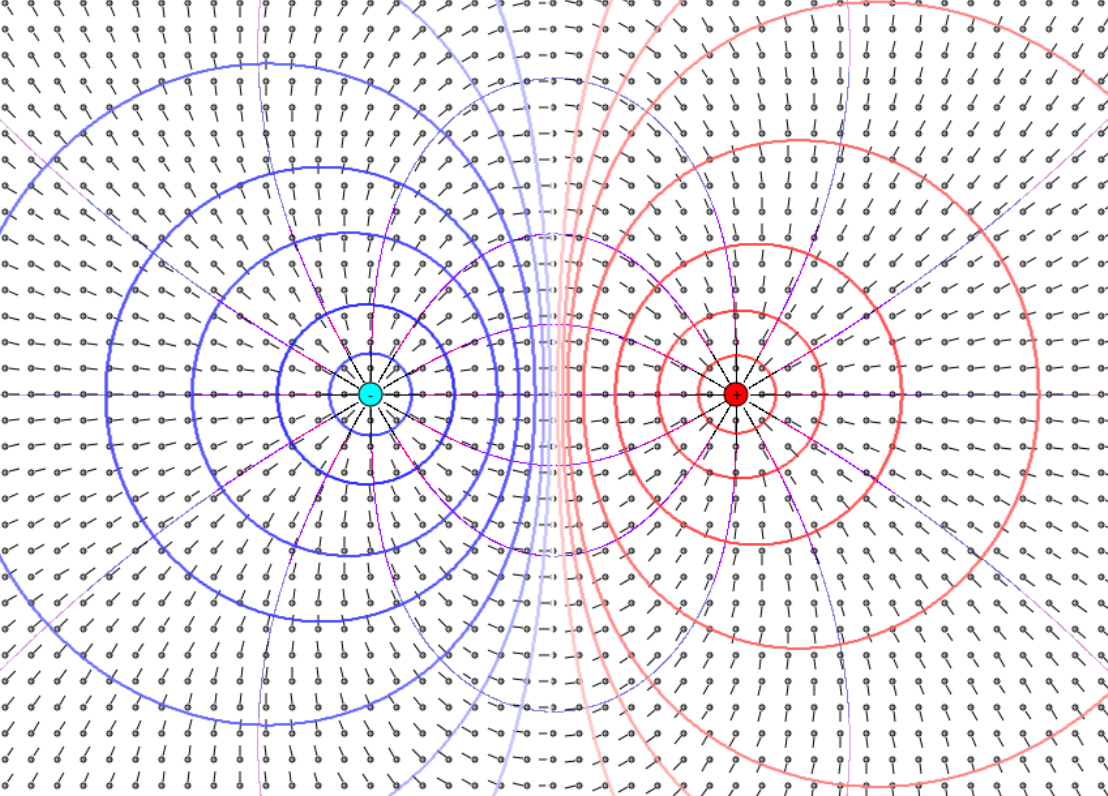
\includegraphics[width=0.6\textwidth]{Aufgaben/Skizze.png}
    \caption{Skizze der Feldlinien sowie Äquipotentiallinien}
    \label{f:times}
    \end{center}
    \end{figure}

\item Auf der x-Achse gilt
\begin{align}
  \vec E(x) &= \frac{q}{4 \pi \epsilon_0}\left(\frac{(x-a)}{|x-a|^3}-\frac{(x+a)}{|x+a|^3}\right)\vec e_x\\
  &=\frac{q}{4 \pi \epsilon_0}\left(\frac{1}{(x-a)^2}-\frac{1}{(x+a)^2}\right)\vec e_x\\
  &=\frac{q}{4 \pi \epsilon_0}\left(\frac{4ax}{(a^2-x^2)^2}\right)\vec e_x\\
  &=\frac{p}{2 \pi \epsilon_0}\left(\frac{x}{(a^2-x^2)^2}\right)\vec e_x\\
  &\approx\frac{p}{2 \pi \epsilon_0}\frac{x}{x^4}\vec e_x\\
  &=\frac{p}{2 \pi \epsilon_0}\frac{1}{x^3}\vec e_x
\end{align}

\item Auf der y-Achse gilt
\begin{align}
\vec E(y) &= \frac{q}{4 \pi \epsilon_0}\left(\frac{\begin{pmatrix} -a\\y \end{pmatrix}}{(a^2+y^2)^{\frac{3}{2}}}-\frac{\begin{pmatrix} a\\y \end{pmatrix}}{(a^2+y^2)^{\frac{3}{2}}}\right)\\
 &= \frac{q}{4 \pi \epsilon_0}\frac{-2a}{(a^2+y^2)^{\frac{3}{2}}} \vec e_x\\
 &= \frac{-p}{4 \pi \epsilon_0}\frac{1}{(a^2+y^2)^{\frac{3}{2}}} \vec e_x\\
 &\approx \frac{-p}{4 \pi \epsilon_0}\frac{1}{y^3} \vec e_x
\end{align}

\end{enumerate}
=======
\item AUfgrund des Superpositionsprinzip, kann das Potential jedes Punktes auf dem Ring aufsummiert werden und erhält so das Gesamtpotential des Rings Rings. Alle Punkte $\vec{x} $ auf der z-Achse haben zum Mittelpunk des Rings einen Abstand z. Daraus ergibt sich der Abstand vom Ring als $\sqrt{R^2 + z^2}$. Die aufsummierte Ladung auf dem Ring ist gerade Q. Dadurch ergibt sich das Potential entlang der z-Achse
\begin{equation}
\phi(z) = \frac{1}{4\pi \epsilon_{0}} \frac{Q}{\sqrt{R^2 + z^2}}
\end{equation}
Im Zentrum des Rings (z = 0) ist das Potential extremal (siehe (b) E(0) = 0).
\begin{equation}
\phi(0) = \frac{1}{4\pi \epsilon_{0}} \frac{-10^{-9}C}{\sqrt{(2.5\cdot 10^{-2}m)^2}} \approx -359.67 V
\end{equation}
\item Das elektrische Feld ergibt sich als Gradient des Potentials. In einer Dimension entspricht das der Ableitung $\frac{\mathrm{d}}{\mathrm{d}z}$. Daraus folgt
\begin{equation}
E(z) = \frac{\mathrm{d}\phi (z)}{\mathrm{d}z}  = \frac{Q}{4\pi \epsilon_{0}} \frac{-z}{(R^2 + z^2)^{\frac{3}{2}}}.
\end{equation}
Die Richtung des Feldes muss aus Symmetriegründen parallel zur z-Achse verlaufen. Als Vektorfeld geschrieben ergibt sich das E-Feld also als
\begin{equation}
\vec{E}(z) = \frac{Q}{4\pi \epsilon_{0}} \frac{-z}{(R^2 + z^2)^{\frac{3}{2}}} \cdot \vec{e_{z}}.
\end{equation}
\item Das Potential ist an der Stelle z = 0 extremal. Die potentielle Energie eines Teilchens mit der Ladung q ist gegeben durch $E(z) = \phi(z) \cdot q$. Für das elektron bedeutet das, dass
\begin{equation}
E_{pot}(0) = \phi(0) \cdot (-e) = 359.67 eV
\end{equation}
das Maximum der potentiellen Energie darstellt. Um dieses Potential zu überwinden muss gelten $E_{kin}(0) \ge 0$, also aufgrund von Energieerhaltung $E_{kin}(\infty) \ge E_{pot}(0) := E_{max} \approx 359.67 eV \approx 5.63 \cdot 10^{-17} J$.
\item In Aufgabenteil (c) haben wir aus der Energieerhaltung hergeleiten, dass gelten musss
\begin{equation}
E_{kin}(\infty) = \frac{m_{e}}{2} v^2 \ge E_{pot}(0) \Leftrightarrow v \ge \sqrt{\frac{2E_{max}}{m_{e}}} \approx 1.125 \cdot 10^{7} \frac{m}{s}
\end{equation}
mit $m_{e}$ die Elektronenmasse.
\end{enumerate}
>>>>>>> 935e2d20a4f70ccba308ca8de5266f2ba2123913
